\documentclass{article}
\usepackage{geometry}
\geometry{letterpaper}
\usepackage{doc}
\usepackage{graphicx}

\title{Peerchat: a Distributed, P2P Communication Network based on Kademlia}
\author{
  Forrest Pieper\\
  Will Drevo\\
  Colin Taylor
}
\date{May 4th, 2014}

\begin{document}

\maketitle

\section{Motivation}
\label{Motivation}

What we today know as the "internet" was started as a US DARPA military project, a network of nodes distributed geographically across the US in order to ensure fault tolerance in the case of a nuclear attack \cite{?}. Today, ironically, many feel the internet has become too centralized. \\

\section{Introduction}

\textit{Peerchat} is a distributed, P2P chat system based on the Kademlia DHT \cite{Maymounkov02} system which adapts Kamdelia to support persistence of users over different IP addresses using the same disk, and a distributed user directory with no central server. \\

To guarantee no central dependencies, Peerchat requires that nodes bootstrap with an explicit IP address of a peer in the Peerchat network in order to be introduced into the routing table and is parameterized by the standard $k$ and $\alpha$ Kademlia parameters. \\

We implemented two main entities for each Peerchat node: \textit{User} and \textit{Node}. This separation ensures that the DHT functionality is separated from the chat protocol. 

\section{Background and Related Work}

A very similar effort is BitTorrent Chat \cite{Goldoor13}, which seeks to leverage the BitTorrent network to also also for personal, anonymous, decentralized communication. The effort has generated excitement due to the already massive user base of BitTorrent, though to date has not been released, nor is planned to be released as open-source. \\

We believe that a truly distributed chat system must be open-source in order to gain acceptance and ensure rigorous third-party audits. Though Peerchat in its current configuration is not secure, we feel that both a starting point and a commitment to open-source is important in a P2P chat client. 

\section{System}

Below is a diagram of a single Peerchat node. 

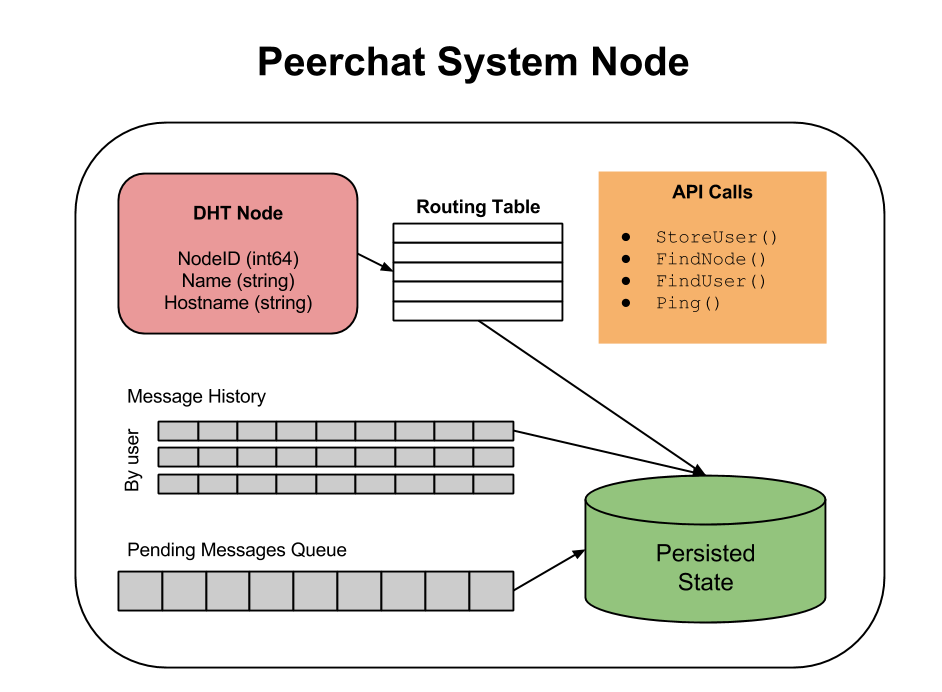
\includegraphics[scale=0.5]{peerchat}

A Peerchat user consists of a number of different routines all working together. A short description of their function is below: \\

Separate threads (goroutines):
\begin{enumerate}
	\item \textit{Message Queuing} \\
	The message queuing routine is what acts when a user submits a message. The user's node sends the message to a queue where it is stored until the Message Sender can deal with the message. Additionally, messages that are being forwarded on in the case of offline messaging are also "piggybacked" into other user's pending messages queue, and await being forwarded to other nodes. 

	\item \textit{Message Sender} \\
	The Message Sending goroutine iterates through the list of recipients with messages to be sent in the User?s queues.  Next, using the DHT, the Message Sender attempts to locate and ping the recipient peer. If the peer is online, the message is sent directly through TCP using an RPC call. If the peer is offline, the Message is sent to the K closest neighbors in the DHT by the XOR metric to increase the chances of message delivery when the recipient happens to come online. 

	\item \textit{Connection Acceptor} \\
The connection acceptor is the Peerchat routine that accepts RPC requests and spins off new goroutines to service them. 

	\item \textit{Periodic Backup} \\
	As well as backing up the system after each received message, Peerchat also backs up it?s message history, routing table, received and seen messages maps, and connection information every 30 seconds. This covers for unpopular nodes who are more often message ?forwarders? than receivers while avoiding spurious serializations to disk. 
\end{enumerate}

\subsection{Persistence}

We persist nodes' state by periodically serializing a user's routing table, messaging log, and other DHT node state to disk.
When a user logs back in, we check for saved data and reconstruct the node.
As long as at least one of the nodes in the saved routing table is still online, the user does not have to specifiy a bootstrap node upon login. 
Otherwise, the user must register their username again and provide a bootstrap node in order to rejoin the system.
If the user's IP address has not changed, we relaunch the node with the old node ID. 
If the user has a new IP address, we generate a new node ID and reorganize the routing table.
This persistence strategy minimizes system disruptions and allows nodes to seamlessly rejoin the network.



\subsection{Offline Usage}

Peerchat assumes online usage, but once a message has failed to send, falls back onto a K closest neighbors forwarding strategy. \\

Upon failure, a node also sends the message to the K nearest nodes around the node, which add the message to their background pending message queues, and attempt in their normal fashion to send them along, keeping the to/from message headers intact. This piggybacked forwarding strategy increases the chances of avoiding a situation in which both nodes continue to miss each other being online, and keeps the conversation going. 

\section{Demonstration}

In addition to a battery of unit tests and simulations, we also present an analysis of the Peerchat's efficiency and and performance under different parameterizations of the system. 

\subsection{User Registration}

colin

\subsection{User Login}

colin 

\subsection{Performance Testing}

will

\subsection{Chat User Interface}

will

\section{Future Work}

Peerchat has many hole that need to be filled before it becomes widely used or trusted. 

Security
UI

\section{Conclusion}

Peerchat is the best, blah, blah.

\begin{thebibliography}{99}
  \bibitem{Maymounkov02}
    %Kademlia
   Maymounkov, Petar and David Mazieres
   ''Kademlia: A Peer-to-peer Information System Based on the XOR Metric''
   \textit{Peer-to-Peer Systems. Springer Berlin Heidelberg}, 2002. 53-65

  \bibitem{Goldoor13}
	%BitTorrent Chat
	Goldoor, Abe
	''Update on BitTorrent Chat.''
	\textit{The BitTorrent Engineering Blog.}, 19 Dec 2013.

\end{thebibliography}

A user contains the API which our Client code uses directly. A user has a username, an Ip address, a message history etc. A user actually sends messages to another user. It also has a pointer to a Node. In this way, a user uses kademlia to find other users's IP addresses and to send offline messages.

In Peerchat, each client, or user, creates a Kademlia node with a 64 int Node ID created from the hash of its IP address. Users find each other by storing a username -> Ip Address mapping in the distributed hash table (DHT). It does so by storing this map at the nearest K closest nodes to the hash of the username. Users call PeerChat's FindUser(username) API, which returns the IP address. Using Kademlia ensures that user?s find each other using at most log(n) hops, where n is the number of nodes (assuming the routing tables are filled in each bucket). 

A user tries to send a message directly, using a background process that keeps sending pending messages until a node replies. In the case of failure, a node also sends the message to the K nearest nodes around the node, which add the message to their background queues. In this way, if the original sender logs out, and the recipient logs back in, the recipient can still receive the message. We call this functionality offline chat.

A node is a Kademlia node as described in the protocol. It is a standalone system which implements it?s 4 main functions: StoreUser, FindNode, FindUser and Ping. It 


\end {document}
